\problemname{Turnering}

\begin{figure}[h!]
  \centering
  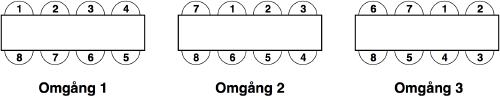
\includegraphics{turnering.png}
\end{figure}

Om man vill ordna t.ex. en bordshockeyturnering där alla möter alla kan man använda sig av ett praktiskt rotationsschema som kallas round robin.
Det går till så att spelarna i den första omgången möter varandra enligt figuren ovan (vi antar att antalet spelare $n$ är jämnt).
När första omgången är klar förflyttar sig alla spelare ett steg medurs, utom spelaren i det nedre vänstra hörnet som hoppas över (därav namnet, man förflyttar sig ``runt'' Robin, d.v.s. den sista spelaren).
Med detta rotationsschema är man garanterad att alla har mött alla precis en gång efter $n-1$ omgångar.

Din uppgift är att skriva ett program som skriver ut vilka spelare som ska möta vilka en viss omgång.

\section*{Indata}
Indata består av två heltal: antal spelare i turneringen (ett jämnt tal $n$ mellan $2$ och $100$) och omgången (mellan $1$ och $n-1$).

\section*{Utdata}
Programmet ska skriva ut $n/2$ rader som beskriver vilka som möter vilka, där varje rad är på formatet \texttt{a-b}.
Ordningen på matcherna spelar ingen roll.
